\documentclass[../main]{subfiles}

\questiontrue
\solutiontrue

\begin{document}
    \ifquestion
   
\section{AstroMagnetism}  

\parte{A}{Relation Between Dipoles}  

\ut{A.1} Consider the planet Pluto II as a sphere with density \( \rho(r) \) at a distance \( r \) from the core and radius \( R \). Recalling that the moment of inertia of a spherical shell is \( \frac{2}{3}MR^2 \), show that the moment of inertia \( I \) of Pluto II around its symmetry axis is:  

\[
I=\frac{8 \pi}{3} \int_0^R r^4 \rho(r) dr
\]  

\ut{A.2} Consider a body (with unspecified geometry) of mass \( M \) and charge \( Q \) with a given distribution of charge and matter relative to a common axis. This distribution follows the criterion: for an element located at \( \vec{r} \), we have \( dq=\kappa dm \), where \( \kappa \) is a constant. Prove the well-known \textit{gyromagnetic ratio}:  

\[
\vec{\mu}=\frac{Q}{2M}\vec{L}
\]  

\ut{A.3} José Lagranja, a great scientist from Pluto III, a neighboring planet of Pluto II, in his book *Principia Plutonis*, shows that Pluto II is a poor conductor (fixed charges) with total charge \( Q \) and satisfies the relation:  

\[
\int_0^Rr^4\rho(r)dr=\mathcal{L}\int_0^Rr^2\rho(r)dr
\]  

where \( \mathcal{L} \) is the Plutonian constant.  

Thus, show that:  

\[
\vec{\mu}=\frac{1}{3}Q\mathcal{L}\vec{\omega}
\]  

Now, consider the following scenario: the planet Pluto II is immersed in an environment with a magnetic field \( \vec{B} \), such that \( |\vec{B}| = 4.87 \) nT, generated by its parent star, Scorp. The planet has a constant density and satisfies the conditions from the previous items, meaning it has mass \( M = 6 \cdot 10^{24} \) kg, a period \( T=25 \) hours, and a total fixed charge \( Q = 5.2 \cdot 10^{21} \) C. The inclination of the planet's rotation axis relative to the magnetic field is \( \theta = 18^\circ24' \), as shown in Figure \ref{fig:eixosBrot}.
	
	\begin{figure}[htpb]
	    \centering
	    

\tikzset{every picture/.style={line width=0.75pt}} %set default line width to 0.75pt        

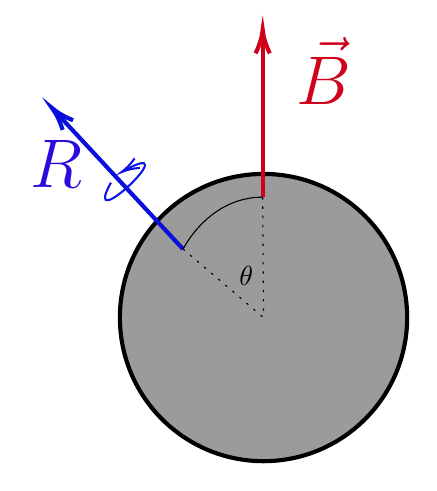
\begin{tikzpicture}[x=0.75pt,y=0.75pt,yscale=-0.8,xscale=0.8]
%uncomment if require: \path (0,408); %set diagram left start at 0, and has height of 408

%Shape: Circle [id:dp33020299009681797] 
\draw  [fill={rgb, 255:red, 155; green, 155; blue, 155 }  ,fill opacity=1 ][line width=1.5]  (244,189.5) .. controls (244,141.73) and (282.73,103) .. (330.5,103) .. controls (378.27,103) and (417,141.73) .. (417,189.5) .. controls (417,237.27) and (378.27,276) .. (330.5,276) .. controls (282.73,276) and (244,237.27) .. (244,189.5) -- cycle ;
%Straight Lines [id:da7248492484832001] 
\draw [color={rgb, 255:red, 208; green, 2; blue, 27 }  ,draw opacity=1 ][line width=1.5]    (330,117) -- (330,19.17) ;
\draw [shift={(330,16.17)}, rotate = 90] [color={rgb, 255:red, 208; green, 2; blue, 27 }  ,draw opacity=1 ][line width=1.5]    (14.21,-4.28) .. controls (9.04,-1.82) and (4.3,-0.39) .. (0,0) .. controls (4.3,0.39) and (9.04,1.82) .. (14.21,4.28)   ;
%Curve Lines [id:da8973244796379132] 
\draw [color={rgb, 255:red, 13; green, 18; blue, 232 }  ,draw opacity=1 ][line width=0.75]    (238.6,108.28) .. controls (219.2,143.12) and (286.04,79.18) .. (246.24,101.18) ;
\draw [shift={(245,101.88)}, rotate = 330.49] [color={rgb, 255:red, 13; green, 18; blue, 232 }  ,draw opacity=1 ][line width=0.75]    (10.93,-3.29) .. controls (6.95,-1.4) and (3.31,-0.3) .. (0,0) .. controls (3.31,0.3) and (6.95,1.4) .. (10.93,3.29)   ;
%Straight Lines [id:da9367992442397037] 
\draw [color={rgb, 255:red, 10; green, 15; blue, 218 }  ,draw opacity=1 ][line width=1.5]    (282,148.22) -- (205.04,65.37) ;
\draw [shift={(203,63.17)}, rotate = 47.11] [color={rgb, 255:red, 10; green, 15; blue, 218 }  ,draw opacity=1 ][line width=1.5]    (14.21,-4.28) .. controls (9.04,-1.82) and (4.3,-0.39) .. (0,0) .. controls (4.3,0.39) and (9.04,1.82) .. (14.21,4.28)   ;
%Shape: Arc [id:dp9976687197606542] 
\draw  [draw opacity=0] (282,148.22) .. controls (292.63,129.31) and (309.96,117) .. (329.53,117) .. controls (329.69,117) and (329.84,117) .. (330,117) -- (329.53,192.12) -- cycle ; \draw   (282,148.22) .. controls (292.63,129.31) and (309.96,117) .. (329.53,117) .. controls (329.69,117) and (329.84,117) .. (330,117) ;  
%Straight Lines [id:da9952920653431763] 
\draw  [dash pattern={on 0.84pt off 2.51pt}]  (282,148.22) -- (330.5,189.5) ;
%Straight Lines [id:da9472800775173769] 
\draw  [dash pattern={on 0.84pt off 2.51pt}]  (330,117) -- (330.5,189.5) ;

% Text Node
\draw (349,19.4) node [anchor=north west][inner sep=0.75pt]  [font=\Huge,color={rgb, 255:red, 208; green, 2; blue, 27 }  ,opacity=1 ]  {$\vec{B}$};
% Text Node
\draw (188.8,81.48) node [anchor=north west][inner sep=0.75pt]  [font=\Huge,color={rgb, 255:red, 40; green, 13; blue, 220 }  ,opacity=1 ]  {$R$};
% Text Node
\draw (314.4,157.08) node [anchor=north west][inner sep=0.75pt]    {$\theta $};


\end{tikzpicture}
	    \caption{Representation of the angular separation between the magnetic field and the planet's axis of rotation}
	    \label{fig:eixosBrot}
	\end{figure}

\ut{A.4} Find the precession period of the equinoxes of this planet. Disregard any other sources of precessional motion.  

\parte{B}{Magnetic GPS}  

José Lagranja, in his quest to complete his pioneering research on the magnetic activity of his planet, sought to locate the magnetic north pole\footnote{At the magnetic north pole, the magnetic field lines enter the surface perpendicularly.} of his planet, which possesses an intrinsic magnetic dipole. The magnetic effect of the planet resembles that of a perfect dipole, which produces an equivalent magnetic field of:
    
    \begin{equation}
    \vec{B}(r, \theta) = \frac{\mu_0 |\vec{\mu}|}{4\pi |\vec{r}|^3}(2\cos(\theta)\hat{r} + \sin(\theta)\hat{\theta})
    \label{eq:magneticfield}
    \end{equation}
    
    %Figure explaining the spherical coordinates
    
    \begin{figure}[htpb]
        \centering
        \tikzset{every picture/.style={line width=0.75pt}}   

    \begin{tikzpicture}[x=0.75pt,y=0.75pt,yscale=-1.2,xscale=1.2]
    
    %Straight Lines [id:da395434186672426] 
    \draw [color={rgb, 255:red, 208; green, 2; blue, 27 }  ,draw opacity=1 ]   (250.5,366.25) -- (250.5,279.75) ;
    \draw [shift={(250.5,277.75)}, rotate = 90] [color={rgb, 255:red, 208; green, 2; blue, 27 }  ,draw opacity=1 ][line width=0.75]    (10.93,-3.29) .. controls (6.95,-1.4) and (3.31,-0.3) .. (0,0) .. controls (3.31,0.3) and (6.95,1.4) .. (10.93,3.29)   ;
    %Straight Lines [id:da4330886082005694] 
    \draw    (250.5,328.75) -- (403.24,246.7) ;
    \draw [shift={(405,245.75)}, rotate = 151.75] [color={rgb, 255:red, 0; green, 0; blue, 0 }  ][line width=0.75]    (10.93,-3.29) .. controls (6.95,-1.4) and (3.31,-0.3) .. (0,0) .. controls (3.31,0.3) and (6.95,1.4) .. (10.93,3.29)   ;
    %Straight Lines [id:da7712952976050258] 
    \draw [color={rgb, 255:red, 17; green, 23; blue, 186 }  ,draw opacity=1 ]   (405,245.75) -- (434.8,227.3) ;
    \draw [shift={(436.5,226.25)}, rotate = 148.24] [color={rgb, 255:red, 17; green, 23; blue, 186 }  ,draw opacity=1 ][line width=0.75]    (10.93,-3.29) .. controls (6.95,-1.4) and (3.31,-0.3) .. (0,0) .. controls (3.31,0.3) and (6.95,1.4) .. (10.93,3.29)   ;
    %Straight Lines [id:da35176934978793417] 
    \draw [color={rgb, 255:red, 17; green, 23; blue, 186 }  ,draw opacity=1 ]   (405,245.75) -- (425.4,276.58) ;
    \draw [shift={(426.5,278.25)}, rotate = 236.51] [color={rgb, 255:red, 17; green, 23; blue, 186 }  ,draw opacity=1 ][line width=0.75]    (10.93,-3.29) .. controls (6.95,-1.4) and (3.31,-0.3) .. (0,0) .. controls (3.31,0.3) and (6.95,1.4) .. (10.93,3.29)   ;
    %Shape: Arc [id:dp7915415121626206] 
    \draw  [draw opacity=0] (250.64,298.75) .. controls (262.13,298.8) and (272.1,305.32) .. (277.1,314.86) -- (250.5,328.75) -- cycle ; \draw   (250.64,298.75) .. controls (262.13,298.8) and (272.1,305.32) .. (277.1,314.86) ;  
    %Straight Lines [id:da9653495168993955] 
    \draw [color={rgb, 255:red, 208; green, 2; blue, 27 }  ,draw opacity=1 ]   (405,245.75) -- (437.59,254.94) -- (451.48,258.86) ;
    \draw [shift={(453.4,259.4)}, rotate = 195.75] [color={rgb, 255:red, 208; green, 2; blue, 27 }  ,draw opacity=1 ][line width=0.75]    (10.93,-3.29) .. controls (6.95,-1.4) and (3.31,-0.3) .. (0,0) .. controls (3.31,0.3) and (6.95,1.4) .. (10.93,3.29)   ;
    
    % Text Node
    \draw (407.5,215.9) node [anchor=north west][inner sep=0.75pt]  [font=\large,color={rgb, 255:red, 17; green, 23; blue, 186 }  ,opacity=1 ]  {$\hat{r}$};
    % Text Node
    \draw (400.5,255.4) node [anchor=north west][inner sep=0.75pt]  [color={rgb, 255:red, 17; green, 23; blue, 186 }  ,opacity=1 ]  {$\hat{\theta }$};
    % Text Node
    \draw (231.6,286.6) node [anchor=north west][inner sep=0.75pt]  [color={rgb, 255:red, 208; green, 2; blue, 27 }  ,opacity=1 ]  {$\vec{\mu }$};
    % Text Node
    \draw (322,266.4) node [anchor=north west][inner sep=0.75pt]  [font=\large]  {$\vec{r}$};
    % Text Node
    \draw (262.73,286.26) node [anchor=north west][inner sep=0.75pt]    {$\theta $};
    % Text Node
    \draw (450.8,233) node [anchor=north west][inner sep=0.75pt]  [color={rgb, 255:red, 208; green, 2; blue, 27 }  ,opacity=1 ]  {$\vec{B}( r,\theta )$};
    
    
    \end{tikzpicture}
        \caption{Scheme representing the magnetic field $\vec{B}$ generated by a dipole $\vec{\mu}$ at a position $\vec{r}$}
        \label{fig:campodedipolo}
    \end{figure}
   
Given that \( \mu_0 \) is the magnetic permeability of vacuum, \( \vec{\mu} \) is the planet's magnetic moment, and \( \vec{r} \) is the position vector of the point where the field is being calculated, with its respective spherical coordinates (\( \hat{r} \) and \( \hat{\theta} \)).  

To find the pole, he devised an experiment: the scientist prepared a short and extremely thin ferromagnetic metal wire and held it by one end. The planet’s magnetism oriented the wire both in the horizontal and vertical planes.  

\ut{B.1} Upon conducting the experiment, the wire tilted about \( 39^\circ 20' \). Find the angular distance between the magnetic north pole and the location of Lagranja's experiment.  

The scientist noticed that the angle between the meridional plane and the vertical plane containing the wire was \( 8^\circ12' \) westward. It is known that Lagranja’s coordinates are \( 17^\circ22' \)N, \( 130^\circ52' \)E.  

\ut{B.2} Determine the coordinates of the magnetic north pole.  

\parte{C}{Rotation of DSCOVR}  

Some time after publishing his book, Lagranja launched a spherical satellite with a radius of \( r=1.62 \) m and mass \( M=570 \) kg, named DSCOVR, and developed software to study his star: JStarViewer. However, a system failure occurred on the satellite, causing it to spin uncontrollably with an angular velocity \( \vec{\omega}(t) \). Just before the failure, the satellite collected data on the magnetic field and the charge flux hitting it, and all this data was transmitted to JStarViewer.
	
	\begin{table}[htpb]
	    \centering
	    \caption{Quantities obtained by satellite and tabulated by JStarViewer}
        \begin{tabular}{c c} 
			\toprule
			Constant & Value \\
			\midrule
			Density of the Stelar Wind & $3.608 \cdot 10^{-23}\ \unit{\gram \per \centi \meter \cubed}$\\
			
			Speed of the Stelar Wind & $313\  \unit{\kilo \meter \per \second}$\\

			Magnetic Field & $4.87\ \unit{\nano \tesla}$\\
			\bottomrule
		\end{tabular}
	    
	    \label{tab:JStarViewer}
	\end{table}

	Consider that initially, the satellite was electrically neutral, that the observed stellar wind consists only of protons, and that the values of the magnetic field, solar wind density, and particle velocity remain constant.  

\ut{C.1} Find the charge accretion rate \( R \) onto the satellite, as well as the total magnetic field in the region.  

\ut{C.2} Determine \( \vec{\omega}(t) \).  

\ut{C.3} Find the time \( t(n) \) elapsed until the satellite completes its \( n \)th precession cycle.
	
	\clearpage
    
    
    \fi
    
    \ifsolution
    
    \section{AstroMagnetism}

Thus, we can express the time derivative of the angular momentum direction as:  

\[
\frac{dL}{dt} = \mu B \sin{\theta}
\]

Since precession is defined as the slow rotation of the angular momentum vector around the external field \( \vec{B} \), the angular velocity of precession \( \Omega_p \) is given by:

\[
\Omega_p = \frac{\tau}{L} = \frac{\mu B \sin{\theta}}{I\omega}
\]

Using the previously derived result:

\[
\mu = \frac{1}{3} Q \mathcal{L} \omega
\]

we substitute into the expression for \( \Omega_p \):

\[
\Omega_p = \frac{\frac{1}{3} Q \mathcal{L} \omega B \sin{\theta}}{I\omega}
\]

Canceling \( \omega \):

\[
\Omega_p = \frac{1}{3} \frac{Q \mathcal{L} B \sin{\theta}}{I}
\]

Since the period of precession \( T_p \) is given by:

\[
T_p = \frac{2\pi}{\Omega_p}
\]

we obtain:

\[
T_p = \frac{6\pi I}{Q \mathcal{L} B \sin{\theta}}
\]

This is the period of precession of Pluto II's equinoxes.
	
	\begin{figure}[htpb]
	    \centering
	    

\tikzset{every picture/.style={line width=0.75pt}} %set default line width to 0.75pt        

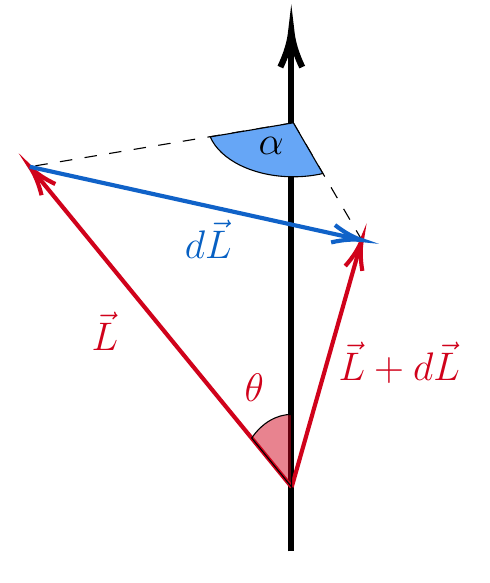
\begin{tikzpicture}[x=0.75pt,y=0.75pt,yscale=-1,xscale=1]
%uncomment if require: \path (0,408); %set diagram left start at 0, and has height of 408

%Straight Lines [id:da5769963883271931] 
\draw [line width=2.25]    (353,346) -- (353,99.17) ;
\draw [shift={(353,95.17)}, rotate = 90] [color={rgb, 255:red, 0; green, 0; blue, 0 }  ][line width=2.25]    (17.49,-5.26) .. controls (11.12,-2.23) and (5.29,-0.48) .. (0,0) .. controls (5.29,0.48) and (11.12,2.23) .. (17.49,5.26)   ;
%Straight Lines [id:da5992729635970626] 
\draw [color={rgb, 255:red, 208; green, 2; blue, 27 }  ,draw opacity=1 ][line width=1.5]    (353.2,315) -- (228.9,163) ;
\draw [shift={(227,160.68)}, rotate = 50.72] [color={rgb, 255:red, 208; green, 2; blue, 27 }  ,draw opacity=1 ][line width=1.5]    (14.21,-4.28) .. controls (9.04,-1.82) and (4.3,-0.39) .. (0,0) .. controls (4.3,0.39) and (9.04,1.82) .. (14.21,4.28)   ;
%Straight Lines [id:da7186499765250391] 
\draw [color={rgb, 255:red, 208; green, 2; blue, 27 }  ,draw opacity=1 ][line width=1.5]    (353.2,315) -- (386.18,198.9) ;
\draw [shift={(387,196.01)}, rotate = 105.86] [color={rgb, 255:red, 208; green, 2; blue, 27 }  ,draw opacity=1 ][line width=1.5]    (14.21,-4.28) .. controls (9.04,-1.82) and (4.3,-0.39) .. (0,0) .. controls (4.3,0.39) and (9.04,1.82) .. (14.21,4.28)   ;
%Straight Lines [id:da3455792312005288] 
\draw  [dash pattern={on 4.5pt off 4.5pt}]  (354,139.51) -- (227,160.68) ;
%Straight Lines [id:da4320797266501242] 
\draw  [dash pattern={on 4.5pt off 4.5pt}]  (354,139.51) -- (387,196.01) ;
%Straight Lines [id:da8934160188362525] 
\draw [color={rgb, 255:red, 16; green, 98; blue, 200 }  ,draw opacity=1 ][fill={rgb, 255:red, 74; green, 144; blue, 226 }  ,fill opacity=1 ][line width=1.5]    (227,160.68) -- (384.07,195.36) ;
\draw [shift={(387,196.01)}, rotate = 192.45] [color={rgb, 255:red, 16; green, 98; blue, 200 }  ,draw opacity=1 ][line width=1.5]    (14.21,-4.28) .. controls (9.04,-1.82) and (4.3,-0.39) .. (0,0) .. controls (4.3,0.39) and (9.04,1.82) .. (14.21,4.28)   ;
%Shape: Pie [id:dp6244208919110701] 
\draw  [fill={rgb, 255:red, 102; green, 166; blue, 246 }  ,fill opacity=1 ] (368.2,163.94) .. controls (363.77,164.95) and (358.99,165.51) .. (354,165.51) .. controls (334.84,165.51) and (318.72,157.36) .. (313.96,146.28) -- (354,139.51) -- cycle ;
%Shape: Pie [id:dp0925790525998933] 
\draw  [fill={rgb, 255:red, 208; green, 2; blue, 27 }  ,fill opacity=0.49 ] (333.94,291.37) .. controls (338.72,284.38) and (345.58,280) .. (353.2,280) -- (353.2,315) -- cycle ;

% Text Node
\draw (336,145) node [anchor=north west][inner sep=0.75pt]  [font=\Large]  {$\alpha$};
% Text Node
\draw (255.5,229.57) node [anchor=north west][inner sep=0.75pt]  [font=\Large,color={rgb, 255:red, 208; green, 2; blue, 27 }  ,opacity=1 ]  {$\vec{L}$};
% Text Node
\draw (374.5,244.07) node [anchor=north west][inner sep=0.75pt]  [font=\Large,color={rgb, 255:red, 208; green, 2; blue, 27 }  ,opacity=1 ]  {$\vec{L} +d\vec{L}$};
% Text Node
\draw (300.5,185.07) node [anchor=north west][inner sep=0.75pt]  [font=\Large,color={rgb, 255:red, 7; green, 96; blue, 195 }  ,opacity=1 ]  {$d\vec{L}$};
% Text Node
\draw (329.2,259.08) node [anchor=north west][inner sep=0.75pt]  [font=\Large,color={rgb, 255:red, 208; green, 2; blue, 27 }  ,opacity=1 ]  {$\theta $};


\end{tikzpicture}
	    \caption{Angular variation of angular momentum due to precession}
	    \label{fig:precess}
	\end{figure}

	The angle of inclination of the ferromagnetic wire in José Lagranja's experiment is given as \( 39^\circ 20' \). This inclination corresponds to the magnetic dip angle, which relates to the latitude \( \lambda \) of the experiment's location via the following equation for a dipole field:

\[
\tan I = 2 \tan \lambda
\]

where \( I \) is the inclination angle. Substituting the given value:

\[
\tan (39^\circ 20') = 2 \tan \lambda
\]

Solving for \( \lambda \):

\[
\lambda = \tan^{-1} \left( \frac{\tan (39^\circ 20')}{2} \right)
\]

This latitude difference \( \lambda \) represents the angular distance between the experiment's location and the magnetic pole. Therefore, we compute:

\[
\Delta \lambda = 90^\circ - \lambda
\]

which provides the latitude of the magnetic north pole.
	
	\begin{figure}[htpb]
	    \centering
	    \tikzset{every picture/.style={line width=0.75pt}} %set default line width to 0.75pt        
    
    \begin{tikzpicture}[x=0.75pt,y=0.75pt,yscale=-1.5,xscale=1.5]
    %uncomment if require: \path (0,598); %set diagram left start at 0, and has height of 598
    
    %Straight Lines [id:da395434186672426] 
    \draw [color={rgb, 255:red, 208; green, 2; blue, 27 }  ,draw opacity=1 ]   (250.5,366.25) -- (250.5,279.75) ;
    \draw [shift={(250.5,277.75)}, rotate = 90] [color={rgb, 255:red, 208; green, 2; blue, 27 }  ,draw opacity=1 ][line width=0.75]    (10.93,-3.29) .. controls (6.95,-1.4) and (3.31,-0.3) .. (0,0) .. controls (3.31,0.3) and (6.95,1.4) .. (10.93,3.29)   ;
    %Straight Lines [id:da4330886082005694] 
    \draw    (250.5,328.75) -- (371.66,259.99) ;
    \draw [shift={(373.4,259)}, rotate = 150.42] [color={rgb, 255:red, 0; green, 0; blue, 0 }  ][line width=0.75]    (10.93,-3.29) .. controls (6.95,-1.4) and (3.31,-0.3) .. (0,0) .. controls (3.31,0.3) and (6.95,1.4) .. (10.93,3.29)   ;
    %Straight Lines [id:da7712952976050258] 
    \draw [color={rgb, 255:red, 17; green, 23; blue, 186 }  ,draw opacity=1 ]   (373.4,259) -- (403.2,240.55) ;
    \draw [shift={(404.9,239.5)}, rotate = 148.24] [color={rgb, 255:red, 17; green, 23; blue, 186 }  ,draw opacity=1 ][line width=0.75]    (10.93,-3.29) .. controls (6.95,-1.4) and (3.31,-0.3) .. (0,0) .. controls (3.31,0.3) and (6.95,1.4) .. (10.93,3.29)   ;
    %Straight Lines [id:da35176934978793417] 
    \draw [color={rgb, 255:red, 17; green, 23; blue, 186 }  ,draw opacity=1 ]   (373.4,259) -- (393.8,289.83) ;
    \draw [shift={(394.9,291.5)}, rotate = 236.51] [color={rgb, 255:red, 17; green, 23; blue, 186 }  ,draw opacity=1 ][line width=0.75]    (10.93,-3.29) .. controls (6.95,-1.4) and (3.31,-0.3) .. (0,0) .. controls (3.31,0.3) and (6.95,1.4) .. (10.93,3.29)   ;
    %Shape: Arc [id:dp7915415121626206] 
    \draw  [draw opacity=0] (250.55,187.05) .. controls (328.62,187.08) and (391.93,250.24) .. (392.2,328.26) -- (250.5,328.75) -- cycle ; \draw   (250.55,187.05) .. controls (328.62,187.08) and (391.93,250.24) .. (392.2,328.26) ;  
    %Straight Lines [id:da9653495168993955] 
    \draw [color={rgb, 255:red, 208; green, 2; blue, 27 }  ,draw opacity=1 ]   (373.4,259) -- (405.99,268.19) -- (419.88,272.11) ;
    \draw [shift={(421.8,272.65)}, rotate = 195.75] [color={rgb, 255:red, 208; green, 2; blue, 27 }  ,draw opacity=1 ][line width=0.75]    (10.93,-3.29) .. controls (6.95,-1.4) and (3.31,-0.3) .. (0,0) .. controls (3.31,0.3) and (6.95,1.4) .. (10.93,3.29)   ;
    %Shape: Arc [id:dp43971402121547] 
    \draw  [draw opacity=0] (250.71,298.68) .. controls (261.73,298.75) and (271.35,304.77) .. (276.51,313.68) -- (250.5,328.75) -- cycle ; \draw   (250.71,298.68) .. controls (261.73,298.75) and (271.35,304.77) .. (276.51,313.68) ;  
    
    % Text Node
    \draw (387.9,220) node [anchor=north west][inner sep=0.75pt]  [font=\large,color={rgb, 255:red, 17; green, 23; blue, 186 }  ,opacity=1 ]  {$\hat{r}$};
    % Text Node
    \draw (370,270) node [anchor=north west][inner sep=0.75pt]  [color={rgb, 255:red, 17; green, 23; blue, 186 }  ,opacity=1 ]  {$\hat{\theta }$};
    % Text Node
    \draw (231.6,286.6) node [anchor=north west][inner sep=0.75pt]  [color={rgb, 255:red, 208; green, 2; blue, 27 }  ,opacity=1 ]  {$\vec{\mu }$};
    % Text Node
    \draw (308.4,312.8) node [anchor=north west][inner sep=0.75pt]  [font=\large]  {$\vec{r}$};
    % Text Node
    \draw (262.73,286.26) node [anchor=north west][inner sep=0.75pt]    {$\theta $};
    % Text Node
    \draw (420,253) node [anchor=north west][inner sep=0.75pt]  [color={rgb, 255:red, 208; green, 2; blue, 27 }  ,opacity=1 ]  {$\vec{B}( r,\theta )$};
    
    
    \end{tikzpicture}
	    \caption{Magnetic Field on the planet's surface as a function of its dipole}
	    \label{fig:magneticfield}
	\end{figure}

Notice that the direction \(\hat{\theta}\) aligns with the ground, while \(\hat{r}\) is perpendicular to it. Thus:

\[
\vec{B}(r, \theta) = \frac{\mu_0 |\vec{\mu}|}{4\pi |\vec{r}|^3}(2\cos(\theta)\hat{r} + \sin(\theta)\hat{\theta})
\]

To calculate the angle of elevation of the wire, observe from the diagram that the tangent of this angle is the ratio between the vertical and horizontal components of the field:

\[
\tan(\kappa) = \frac{2\cos(\theta)}{\sin(\theta)} = 2 \cot(\theta)
\]

Since \(\kappa = 39^\circ 20 '\), as the wire tilted, it follows that \(\theta = 67^\circ43'\).

\ut{B.2} Analyzing the positioning diagram on the planet, we can construct the following spherical triangle:
	
	\begin{figure}[htpb]
	    \centering
    \tikzset{every picture/.style={line width=0.75pt}} %set default line width to 0.75pt        
    
    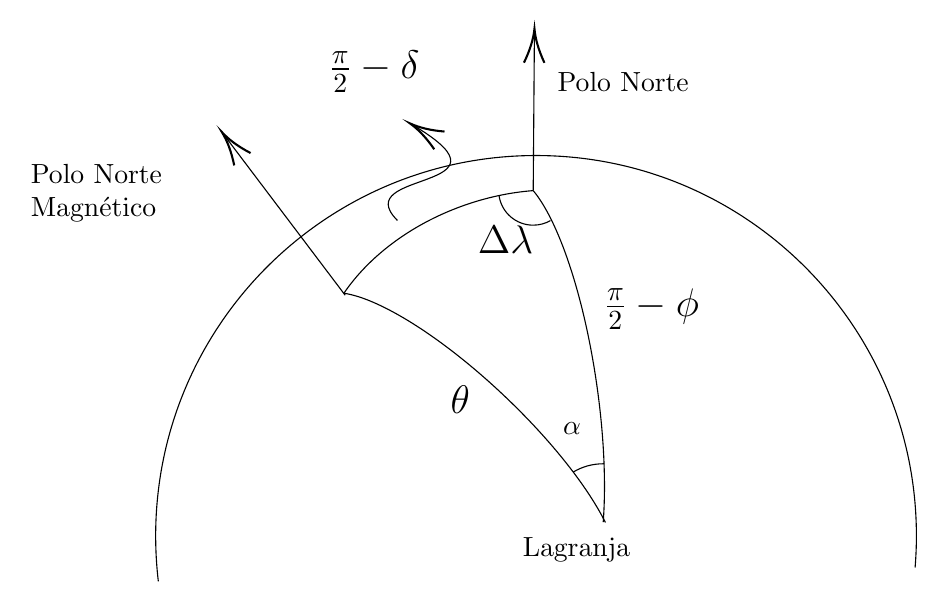
\begin{tikzpicture}[x=0.75pt,y=0.75pt,yscale=-1.5,xscale=1.5]
    %uncomment if require: \path (0,598); %set diagram left start at 0, and has height of 598
    
    %Straight Lines [id:da9758362499244775] 
    \draw    (239.8,223) -- (201.41,172.2) ;
    \draw [shift={(200.2,170.6)}, rotate = 52.92] [color={rgb, 255:red, 0; green, 0; blue, 0 }  ][line width=0.75]    (10.93,-3.29) .. controls (6.95,-1.4) and (3.31,-0.3) .. (0,0) .. controls (3.31,0.3) and (6.95,1.4) .. (10.93,3.29)   ;
    %Straight Lines [id:da82349494366702] 
    \draw    (300.2,189.4) -- (300.58,139.4) ;
    \draw [shift={(300.6,137.4)}, rotate = 90.44] [color={rgb, 255:red, 0; green, 0; blue, 0 }  ][line width=0.75]    (10.93,-3.29) .. controls (6.95,-1.4) and (3.31,-0.3) .. (0,0) .. controls (3.31,0.3) and (6.95,1.4) .. (10.93,3.29)   ;
    %Shape: Arc [id:dp985124533981492] 
    \draw  [draw opacity=0] (300.2,189.4) .. controls (308.25,199.02) and (316.36,222.67) .. (320.5,250.98) .. controls (322.97,267.84) and (323.61,283.52) .. (322.68,295.88) -- (302.16,253.66) -- cycle ; \draw   (300.2,189.4) .. controls (308.25,199.02) and (316.36,222.67) .. (320.5,250.98) .. controls (322.97,267.84) and (323.61,283.52) .. (322.68,295.88) ;  
    %Shape: Arc [id:dp755986652761764] 
    \draw  [draw opacity=0] (239.39,222.36) .. controls (251.06,224.08) and (271.31,236.7) .. (291.11,255.51) .. controls (306.21,269.85) and (317.73,284.64) .. (323.38,295.98) -- (278.35,268.95) -- cycle ; \draw   (239.39,222.36) .. controls (251.06,224.08) and (271.31,236.7) .. (291.11,255.51) .. controls (306.21,269.85) and (317.73,284.64) .. (323.38,295.98) ;  
    %Shape: Arc [id:dp24293333275149953] 
    \draw  [draw opacity=0] (239.39,222.36) .. controls (247.34,210.71) and (260.6,200.46) .. (277.21,194.42) .. controls (284.95,191.61) and (292.73,189.97) .. (300.2,189.4) -- (292.34,236.06) -- cycle ; \draw   (239.39,222.36) .. controls (247.34,210.71) and (260.6,200.46) .. (277.21,194.42) .. controls (284.95,191.61) and (292.73,189.97) .. (300.2,189.4) ;  
    %Shape: Arc [id:dp35859895055214586] 
    \draw  [draw opacity=0] (305.74,199.02) .. controls (304.11,199.96) and (302.22,200.5) .. (300.2,200.5) .. controls (294.64,200.5) and (290.04,196.42) .. (289.23,191.09) -- (300.2,189.4) -- cycle ; \draw   (305.74,199.02) .. controls (304.11,199.96) and (302.22,200.5) .. (300.2,200.5) .. controls (294.64,200.5) and (290.04,196.42) .. (289.23,191.09) ;  
    %Shape: Arc [id:dp23954250567664204] 
    \draw  [draw opacity=0] (313.01,279.82) .. controls (315.84,278.12) and (319.14,277.14) .. (322.68,277.14) .. controls (322.79,277.14) and (322.9,277.14) .. (323.01,277.14) -- (322.68,295.88) -- cycle ; \draw   (313.01,279.82) .. controls (315.84,278.12) and (319.14,277.14) .. (322.68,277.14) .. controls (322.79,277.14) and (322.9,277.14) .. (323.01,277.14) ;  
    %Curve Lines [id:da9525995981498676] 
    \draw    (256.6,199) .. controls (240.45,182.85) and (296.86,189.59) .. (262.25,168.77) ;
    \draw [shift={(260.6,167.8)}, rotate = 30.07] [color={rgb, 255:red, 0; green, 0; blue, 0 }  ][line width=0.75]    (10.93,-3.29) .. controls (6.95,-1.4) and (3.31,-0.3) .. (0,0) .. controls (3.31,0.3) and (6.95,1.4) .. (10.93,3.29)   ;
    %Shape: Arc [id:dp7819560060471606] 
    \draw  [draw opacity=0] (179.79,314.92) .. controls (179.22,310.12) and (178.93,305.25) .. (178.93,300.3) .. controls (178.93,232.82) and (233.62,178.13) .. (301.1,178.13) .. controls (368.58,178.13) and (423.28,232.82) .. (423.28,300.3) .. controls (423.28,303.72) and (423.13,307.11) .. (422.86,310.46) -- (301.1,300.3) -- cycle ; \draw   (179.79,314.92) .. controls (179.22,310.12) and (178.93,305.25) .. (178.93,300.3) .. controls (178.93,232.82) and (233.62,178.13) .. (301.1,178.13) .. controls (368.58,178.13) and (423.28,232.82) .. (423.28,300.3) .. controls (423.28,303.72) and (423.13,307.11) .. (422.86,310.46) ;  
    
    % Text Node
    \draw (322,220) node [anchor=north west][inner sep=0.75pt]  [font=\Large]  {$\frac{\pi }{2} -\phi $};
    % Text Node
    \draw (281.6,199.8) node [anchor=north west][inner sep=0.75pt]  [font=\Large]  {$\Delta \lambda $};
    % Text Node
    \draw (233.6,143.8) node [anchor=north west][inner sep=0.75pt]  [font=\Large]  {$\frac{\pi }{2} -\delta $};
    % Text Node
    \draw (272.8,251.2) node [anchor=north west][inner sep=0.75pt][font = \Large]    {$\theta $};
    % Text Node
    \draw (309,263) node [anchor=north west][inner sep=0.75pt]   {$\alpha $};
    % Text Node
    \draw (307.2,150.4) node [anchor=north west][inner sep=0.75pt]   [align=left] {Polo Norte};
    % Text Node
    \draw (138,180) node [anchor=north west][inner sep=0.75pt]   [align=left] {Polo Norte\\Magnético};
    % Text Node
    \draw (296,300) node [anchor=north west][inner sep=0.75pt]   [align=left] {Lagranja};
    
    
    \end{tikzpicture}
	\caption{Spherical positions of the magnetic north pole, north pole and Lagranja}
	\label{fig:geopos}
	\end{figure}

Notice that the wire will align with the plane that passes through Lagranja and contains the Magnetic North Pole. Thus, the angle between the wire and the meridian plane (which passes through the Planetary North Pole) is precisely the angle \(\alpha\) as represented in figure \ref{fig:geopos}. By the spherical law of cosines, it is known that:

\[
\cos\left(\frac{\pi}{2} - \delta\right) = \cos(\theta)\cos\left(\frac{\pi}{2} - \phi\right) + \sin(\theta)\sin\left(\frac{\pi}{2} - \phi\right)\cos(\alpha)
\]

\[
\therefore \sin(\delta) = \cos(\theta)\sin(\phi) + \sin(\theta)\cos(\phi)\cos(\alpha)
\]

Thus, we can conclude that the latitude of the magnetic pole is \(\delta = 80^\circ 51'\). Now, by the spherical law of sines, it is possible to find the relation for \(\Delta \lambda\):

\[
\frac{\sin(\Delta \lambda)}{\sin(\theta)} = \frac{\sin(\alpha)}{\sin\left(\frac{\pi}{2} - \delta\right)}
\]

\[
\therefore \Delta \lambda = 56^\circ 5'
\]

Assume that the coordinate system of Pluto III is similar to Earth's (longitude is counted from left to right from an observer in space). Thus, it can be seen that the magnetic pole is \(\Delta \lambda\) degrees west of Lagranja's position. Therefore, simply subtract \(\Delta \lambda\) from the researcher's longitude: \(\lambda_{PMN} = 130^\circ 52' - 56^\circ 5' = 74^\circ 47'\).

Thus, the coordinates of the magnetic north pole are: \(80^\circ 51'N\) \(74^\circ 47'E\).

\parte{C}{Rotation of the DSCOVR}

\ut{C.1} Given the particle density \(\rho\), the mass of the particles \(\mu\) (the particle number density is therefore \(\dfrac{\rho}{\mu}\)), and the velocity of the particles \(v\), consider the number of particles that will hit the satellite within an interval \(dt\). These particles are within a cylinder with the area of the satellite and are at most a distance \(vdt\) from the satellite, as shown in figure \ref{fig:vazaocharge}.
	
	\begin{figure}[htpb]
	    \centering
	    

\tikzset{every picture/.style={line width=0.75pt}} %set default line width to 0.75pt        

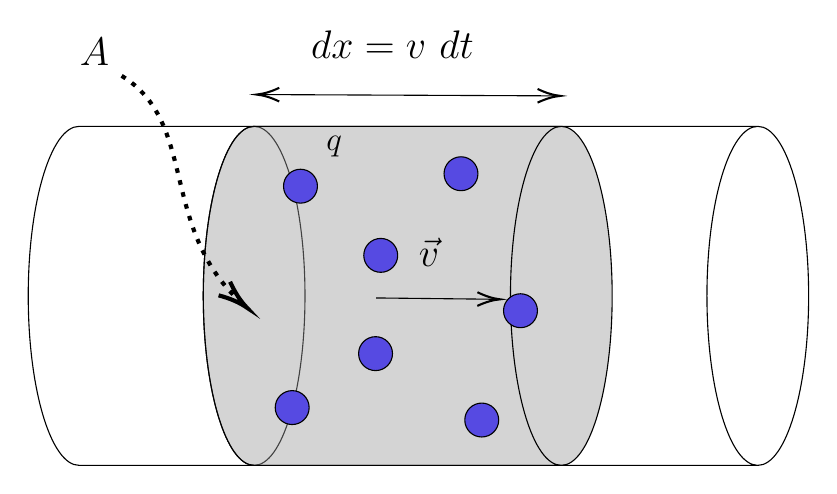
\begin{tikzpicture}[x=0.75pt,y=0.75pt,yscale=-1,xscale=1]
%uncomment if require: \path (0,408); %set diagram left start at 0, and has height of 408

%Shape: Can [id:dp19306472541477993] 
\draw   (473.83,281.34) -- (146.83,281.34) .. controls (133.3,281.34) and (122.33,244.78) .. (122.33,199.68) .. controls (122.33,154.57) and (133.3,118.01) .. (146.83,118.01) -- (473.83,118.01) .. controls (487.36,118.01) and (498.33,154.57) .. (498.33,199.68) .. controls (498.33,244.78) and (487.36,281.34) .. (473.83,281.34) .. controls (460.3,281.34) and (449.33,244.78) .. (449.33,199.68) .. controls (449.33,154.57) and (460.3,118.01) .. (473.83,118.01) ;
%Shape: Ellipse [id:dp3342488937535777] 
\draw   (206.67,199.68) .. controls (206.67,154.57) and (217.64,118.01) .. (231.17,118.01) .. controls (244.7,118.01) and (255.67,154.57) .. (255.67,199.68) .. controls (255.67,244.78) and (244.7,281.34) .. (231.17,281.34) .. controls (217.64,281.34) and (206.67,244.78) .. (206.67,199.68) -- cycle ;
%Shape: Can [id:dp318933498571764] 
\draw  [fill={rgb, 255:red, 155; green, 155; blue, 155 }  ,fill opacity=0.43 ] (379.17,281.34) -- (231.17,281.34) .. controls (217.64,281.34) and (206.67,244.78) .. (206.67,199.68) .. controls (206.67,154.57) and (217.64,118.01) .. (231.17,118.01) -- (379.17,118.01) .. controls (392.7,118.01) and (403.67,154.57) .. (403.67,199.68) .. controls (403.67,244.78) and (392.7,281.34) .. (379.17,281.34) .. controls (365.64,281.34) and (354.67,244.78) .. (354.67,199.68) .. controls (354.67,154.57) and (365.64,118.01) .. (379.17,118.01) ;
%Straight Lines [id:da579008132852971] 
\draw    (234.33,102.69) -- (376.67,103.32) ;
\draw [shift={(378.67,103.33)}, rotate = 180.26] [color={rgb, 255:red, 0; green, 0; blue, 0 }  ][line width=0.75]    (10.93,-3.29) .. controls (6.95,-1.4) and (3.31,-0.3) .. (0,0) .. controls (3.31,0.3) and (6.95,1.4) .. (10.93,3.29)   ;
\draw [shift={(232.33,102.68)}, rotate = 0.26] [color={rgb, 255:red, 0; green, 0; blue, 0 }  ][line width=0.75]    (10.93,-3.29) .. controls (6.95,-1.4) and (3.31,-0.3) .. (0,0) .. controls (3.31,0.3) and (6.95,1.4) .. (10.93,3.29)   ;
%Curve Lines [id:da9069828281940029] 
\draw [line width=1.5]  [dash pattern={on 1.69pt off 2.76pt}]  (167.33,93.67) .. controls (204.44,116.33) and (184.94,167.12) .. (225.76,203.68) ;
\draw [shift={(227.67,205.34)}, rotate = 220.24] [color={rgb, 255:red, 0; green, 0; blue, 0 }  ][line width=1.5]    (14.21,-4.28) .. controls (9.04,-1.82) and (4.3,-0.39) .. (0,0) .. controls (4.3,0.39) and (9.04,1.82) .. (14.21,4.28)   ;
%Shape: Circle [id:dp782790970823624] 
\draw  [fill={rgb, 255:red, 86; green, 74; blue, 226 }  ,fill opacity=1 ] (245.33,146.83) .. controls (245.33,142.32) and (248.99,138.67) .. (253.5,138.67) .. controls (258.01,138.67) and (261.67,142.32) .. (261.67,146.83) .. controls (261.67,151.34) and (258.01,155) .. (253.5,155) .. controls (248.99,155) and (245.33,151.34) .. (245.33,146.83) -- cycle ;
%Shape: Circle [id:dp8043663665132939] 
\draw  [fill={rgb, 255:red, 86; green, 74; blue, 226 }  ,fill opacity=1 ] (351.33,206.83) .. controls (351.33,202.32) and (354.99,198.67) .. (359.5,198.67) .. controls (364.01,198.67) and (367.67,202.32) .. (367.67,206.83) .. controls (367.67,211.34) and (364.01,215) .. (359.5,215) .. controls (354.99,215) and (351.33,211.34) .. (351.33,206.83) -- cycle ;
%Shape: Circle [id:dp7729762463157726] 
\draw  [fill={rgb, 255:red, 86; green, 74; blue, 226 }  ,fill opacity=1 ] (241.33,253.5) .. controls (241.33,248.99) and (244.99,245.33) .. (249.5,245.33) .. controls (254.01,245.33) and (257.67,248.99) .. (257.67,253.5) .. controls (257.67,258.01) and (254.01,261.67) .. (249.5,261.67) .. controls (244.99,261.67) and (241.33,258.01) .. (241.33,253.5) -- cycle ;
%Shape: Circle [id:dp9375817268492423] 
\draw  [fill={rgb, 255:red, 86; green, 74; blue, 226 }  ,fill opacity=1 ] (332.67,259.5) .. controls (332.67,254.99) and (336.32,251.33) .. (340.83,251.33) .. controls (345.34,251.33) and (349,254.99) .. (349,259.5) .. controls (349,264.01) and (345.34,267.67) .. (340.83,267.67) .. controls (336.32,267.67) and (332.67,264.01) .. (332.67,259.5) -- cycle ;
%Shape: Circle [id:dp20056720256950245] 
\draw  [fill={rgb, 255:red, 86; green, 74; blue, 226 }  ,fill opacity=1 ] (322.67,140.83) .. controls (322.67,136.32) and (326.32,132.67) .. (330.83,132.67) .. controls (335.34,132.67) and (339,136.32) .. (339,140.83) .. controls (339,145.34) and (335.34,149) .. (330.83,149) .. controls (326.32,149) and (322.67,145.34) .. (322.67,140.83) -- cycle ;
%Shape: Circle [id:dp18740812919382854] 
\draw  [fill={rgb, 255:red, 86; green, 74; blue, 226 }  ,fill opacity=1 ] (284,180.17) .. controls (284,175.66) and (287.66,172) .. (292.17,172) .. controls (296.68,172) and (300.33,175.66) .. (300.33,180.17) .. controls (300.33,184.68) and (296.68,188.33) .. (292.17,188.33) .. controls (287.66,188.33) and (284,184.68) .. (284,180.17) -- cycle ;
%Shape: Circle [id:dp6072127200025121] 
\draw  [fill={rgb, 255:red, 86; green, 74; blue, 226 }  ,fill opacity=1 ] (281.5,227.51) .. controls (281.5,223) and (285.16,219.34) .. (289.67,219.34) .. controls (294.18,219.34) and (297.83,223) .. (297.83,227.51) .. controls (297.83,232.02) and (294.18,235.68) .. (289.67,235.68) .. controls (285.16,235.68) and (281.5,232.02) .. (281.5,227.51) -- cycle ;
%Straight Lines [id:da19042822817218408] 
\draw    (290,200.68) -- (347.67,201.32) ;
\draw [shift={(349.67,201.34)}, rotate = 180.64] [color={rgb, 255:red, 0; green, 0; blue, 0 }  ][line width=0.75]    (10.93,-3.29) .. controls (6.95,-1.4) and (3.31,-0.3) .. (0,0) .. controls (3.31,0.3) and (6.95,1.4) .. (10.93,3.29)   ;

% Text Node
\draw (257.33,70.73) node [anchor=north west][inner sep=0.75pt]  [font=\Large]  {$dx=v\ dt$};
% Text Node
\draw (146,74.4) node [anchor=north west][inner sep=0.75pt]  [font=\Large]  {$A$};
% Text Node
\draw (309.33,170.74) node [anchor=north west][inner sep=0.75pt]  [font=\Large]  {$\vec{v}$};
% Text Node
\draw (264.67,121.41) node [anchor=north west][inner sep=0.75pt]  [font=\large]  {$q$};


\end{tikzpicture}
	    \caption{Representation of charge flow in space}
	    \label{fig:vazaocharge}
	\end{figure}

	
Therefore, the charge that reaches the satellite is: \(\dfrac{\rho}{\mu}qAvdt\), where \(q\) is the charge of each particle. Therefore:

\[
R=\frac{\rho \pi r^2 v q}{\mu}
\]

Since the effective cross-sectional area of the satellite is \(\pi r^2\).

Substituting the values, we find:

\[
R=8.916 \cdot 10^{-6} \, \text{C} \cdot \text{s}^{-1}
\]

\ut{C.2} Define:

\[
\vec{\omega}(t)=\omega_x(t)\hat{i}+\omega_y(t)\hat{j}+\omega_z(t)\hat{k}
\]

Let us define the coordinate space based on the position of the magnetic field (since this is the invariant factor in the problem):

\[
\vec{B}=B\hat{k}
\]

\[
\vec{L}=I\vec{\omega}
\]

The charge of the body grows linearly with the relation \(Q(t)=Rt\), therefore:

\[
\vec{\mu}(t)=\frac{Rt}{2M}I\vec{\omega(t)}
\]

Considering the torque exerted by the field:

\[
\vec{\tau}=I\vec{\alpha}=\vec{\mu} \times \vec{B}
\]

\[
\vec{\alpha}=\frac{Rt}{2M}\vec{\omega(t)}\times\vec{B}
\]

\[
\vec{\alpha}=\frac{d\vec{\omega}}{dt}
\]

By the well-known relation for finding the cross product between two vectors:

\[
\vec{\omega}(t)\times\vec{B}=	
\begin{Vmatrix}
	\hat{i} & \hat{j} & \hat{k} \\
	\omega_x(t) & \omega_y(t) & \omega_z(t) \\
	0 & 0 & B \\
\end{Vmatrix}
\]

\[
\vec{\omega}(t)\times\vec{B}=	\omega_y(t)B\hat{i}-\omega_x(t)B\hat{j}
\]

\[
\frac{d\omega_x(t)}{dt}\hat{i}+\frac{d\omega_y(t)}{dt}\hat{j}+\frac{d\omega_z(t)}{dt}\hat{k}=\frac{Rt}{2M}	\omega_y(t)B\hat{i}-\frac{Rt}{2M}\omega_x(t)B\hat{j}
\]

Since the unit vectors \(\hat{i}\), \(\hat{j}\), and \(\hat{k}\) are linearly independent, for the vectors to be equal, their components along each axis must be equal:

\[
\begin{cases}
	\frac{d\omega_z(t)}{dt}=0 \\
	\frac{d\omega_x(t)}{dt}=\frac{Rt}{2M}	\omega_y(t)B\\	\frac{d\omega_y(t)}{dt}=-\frac{Rt}{2M}\omega_x(t)B\\
\end{cases}
\]

Dividing the last two equations:

\[
\omega_x(t)d\omega_x(t)=-\omega_y(t)d\omega_y(t)
\]

Integrating and rearranging:

\[
\omega^2_x(t)+\omega^2_y(t)=\omega_0^2
\]

Where \(\omega_0\) is an integration constant. Having found the relationship between \(\omega_x\) and \(\omega_y\), let us proceed:

\[
d\omega_y(t)=d\sqrt{\omega^2_0-\omega^2_x(t)}=\frac{-2\omega_x(t)d\omega_x(t)}{2\sqrt{\omega^2_0-\omega^2_x(t)}}
\]

Substituting this result into the last equation of the system:

\[
\frac{d\omega_x(t)}{\sqrt{\omega^2_0-\omega^2_x(t)}}=\frac{Rt}{2M}Bdt
\]

\[
\int_{\omega_{x,0}}^{\omega_{x}(t)}\frac{d\omega_x(t)}{\sqrt{\omega^2_0-\omega^2_x(t)}}=\frac{Rt^2}{4M}B
\]

Substituting \(\omega_x(t)=\omega_0\sin{(y)}\), and knowing that: \(d\omega_x(t)=\omega_0\cos{(y)}dy\):

\[
\int_{y_0}^{y}\frac{\cos{(y)}dy}{\sqrt{1-\sin^2{(y)}}}=\frac{Rt^2}{4M}B
\]

\[
y-y_0=\frac{Rt^2}{4M}B=\arcsin{\left( \frac{\omega_x(t)}{\omega_0}\right) }-\arcsin{\left( \frac{\omega_{x,0}}{\omega_0}\right) }
\]

\[
\omega_x(t)=\omega_0\sin{\left( \frac{Rt^2}{4M}B + \arcsin{ \left(  \frac{\omega_{x,0}}{\omega_0} \right)} \right)}
\]

\[
\omega_y(t)=\omega_0\cos{\left( \frac{Rt^2}{4M}B + \arccos{ \left(  \frac{\omega_{y,0}}{\omega_0} \right)} \right)}
\]

\[
\omega_z(t)=\omega_{z,0}
\]

Finally:

\[
\vec{\omega}(t)=\omega_0\sin{\left( \frac{Rt^2}{4M}B + \arcsin{ \left(  \frac{\omega_{x,0}}{\omega_0} \right)} \right)}\hat{i} + \omega_0\cos{\left( \frac{Rt^2}{4M}B + \arccos{ \left(  \frac{\omega_{y,0}}{\omega_0} \right)} \right)} \hat{j} + \omega_{z,0}\hat{k}
\]

\ut{C.3} Note that for the satellite to complete a full precessional rotation, the angular velocity configuration must return to the same value, which occurs when the argument of the trigonometric functions increases by \(2\pi\) (a full rotation). Therefore, for the \(n\)-th rotation: \(\Delta \theta =2n\pi\), thus:

\[
\frac{Rt^2(n)}{4M}B=2n\pi
\]

Therefore:

\[
t(n)=\sqrt{\frac{8M\pi}{RB}}\sqrt{n}
\]

Substituting the values:

\[
t(n)=18.214\sqrt{n} \, \text{years}
\]

\textbf{BONUS:} The period for the \(n\)-th rotation is given by:

\[
P(n) = \Delta t(n) = t(n+1) - t(n) = 18.214(\sqrt{n+1} - \sqrt{n})
\]

For large values of \(n\), Bernoulli's approximation can be used: \(\sqrt{n+1} = \sqrt{n} \sqrt{1+\dfrac{1}{n}} \approx \sqrt{n}\left(1+\dfrac{1}{2n}\right)\):

\[
P(n) = 18.214\frac{\sqrt{n}}{2n} = \frac{9.107}{\sqrt{n}}
\]

This reveals that the satellite rotates faster and faster, as the precessional period decreases with the factor \(\sqrt{n}\).

	
	\clearpage
    
    
    \fi
\end{document}
